\documentclass{article}
\usepackage{fleqn}
\usepackage{epsf}
\usepackage{aima2e-slides}
\usepackage{graphicx}
\usepackage{listings}

\usepackage[landscape]{geometry}

%\usepackage{amsmath}
\usepackage{amssymb}

\newcommand{\mm}{\!\!-\!\!}
\newcommand{\prompt}{$> \ $}
\newcommand{\rep}[1]{\ulcorner #1 \urcorner}

\begin{document}

\begin{huge}
\titleslide{Chapter 4. State \\ (Essentials of Programming Languages)}{Kwanghoon Choi \\ \ \\ Software Languages and Systems Laboratory\\ Chonnam National University}

\sf

%%%%%%%%%%%% Slide %%%%%%%%%%%%%%%%%%%%%%%%%%%%%%%%%%%%%%%%%%%%%%%%%%%
\heading{Outline}


\blob Computational Effects

\blob EXPLICIT-REFS: A Language with Explicit References 

\blob IMPLICIT-REFS: A Language with Implicit References 

\blob MUTABLE-PAIRS: A Language with Mutable Pairs

\blob Parameter-Passing Variations

%%%%%%%%%%%% Slide %%%%%%%%%%%%%%%%%%%%%%%%%%%%%%%%%%%%%%%%%%%%%%%%%%%
\heading{4.1 Computational Effects}

A computation produces a value possibly with effects (e.g., read, print, alter the state of memory or a file system) 

Here, we focus on a single effect: assignment to a location in memory \al
   - binding vs. assignment

Store (i.e., memory): a finite map from {\it locations} to so called the {\it storable values} \al
   - Env.: a finite map from variables to locations

Reference: a data structure that represents a location \al
   - L-values (references), R-values (expressed values)

Two designs for a language with a store \al
   - explicit references and implicit references

%%%%%%%%%%%% Slide %%%%%%%%%%%%%%%%%%%%%%%%%%%%%%%%%%%%%%%%%%%%%%%%%%%
\heading{4.2 EXPLICIT-REFS: A Lang. with Expl. Refs.}

\blob Examples in EXPLICIT-REFS

\begin{lstlisting}[language=Lisp]
let x = newref (0) in  
letrec 
  even(dummy) = if zero? (deref(x)) then 1
    else begin
           setref(x, -(deref(x), 1));
           (odd 888)
         end
  odd(dummy) = if zero? (deref(x)) then 0
    else begin 
           setref(x, -(deref(x), 1));
           (even 888)
         end
in begin setref(x,13); (odd 888) end
\end{lstlisting}

%%%%%%%%%%%% Slide %%%%%%%%%%%%%%%%%%%%%%%%%%%%%%%%%%%%%%%%%%%%%%%%%%%
\heading{4.2 EXPLICIT-REFS: A Lang. with Expl. Refs.}

\blob Examples in EXPLICIT-REFS (cont.)

\begin{lstlisting}[language=Lisp]
let g = let counter = newref(0) in  
          proc (dummy) 
            begin
             setref(counter, -(deref(counter), -1));
             deref(counter)
            end
in let a = (g 11)
    in let b = (g 11)
        in -(a, b)
\end{lstlisting}

Question. Do Exercise 4.1

%%%%%%%%%%%% Slide %%%%%%%%%%%%%%%%%%%%%%%%%%%%%%%%%%%%%%%%%%%%%%%%%%%
\heading{4.2 EXPLICIT-REFS: A Lang. with Expl. Refs.}

Three new operations {\it newref}, {\it deref}, and {\it setref} to create and use references \al
- In odd/even, let x = newref(0) in ...,  deref(x), setref(x, 13) \al
- In counter, let counter = newref(0) in ..., setref(counter, -(deref(counter), -1))  

Question. How do you write the three operations in your favorite languages such as C, C++, and Java?

References as a new kind of expressed values \al
- ExpVal = Int + Bool + Proc + Ref(Expval) \al
- DenVal = ExpVal

Question. Explain the behavior of ``newref (newref (0))".

%%%%%%%%%%%% Slide %%%%%%%%%%%%%%%%%%%%%%%%%%%%%%%%%%%%%%%%%%%%%%%%%%%
\heading{4.2.1 Store-Passing Specifications}

In EXPLICIT-REFS, any expression may have an effect. To specify these effects, we need to describe what store should be used for
each evaluation and how each evaluation can modify the store.

Store $\sigma$: a finite map from locations to (storable) values \al
- $[l=v]\sigma$ is a store $\sigma$ except  that location $l$ is mapped to $v$ \al
- A particular of value of $\sigma$ is called the {\it state} of the store

A store-passing specification: 
Expression $exp$, evaluated in environment $\rho$ and with the store in state $\sigma_{init}$, 
returns the value $val$ and leaves the store in a possibly different state $\sigma$. \al
- (value-of $exp$ $\rho$ $\sigma_{init}$) = ($val$, $\sigma$)

%%%%%%%%%%%% Slide %%%%%%%%%%%%%%%%%%%%%%%%%%%%%%%%%%%%%%%%%%%%%%%%%%%
\heading{4.2.1 Store-Passing Specifications (Cont.)}

A store-passing specification: (value-of $exp$ $\rho$ $\sigma_{init}$) = ($val$, $\sigma$)

For const-exp: \al
(value-of (const-exp $n$) $\rho$ $\sigma$) = ($n$, $\sigma$) \al
\ \al
Note that const-exp is an effect-free operation. \al

For diff-exp: \al
\begin{tabular}{l}
(value-of $exp_1$ $\rho$ $\sigma_0$) = ($val_1$, $\sigma_1$) \\ 
(value-of $exp_2$ $\rho$ $\sigma_1$) = ($val_2$, $\sigma_2$) \\ \hline
(value-of (diff-exp $exp_1$ $exp_2$) $\rho$ $\sigma_0$) = ($\ceiling{\floor{val_1}-\floor{val_2}}$, $\sigma_2$) 
\end{tabular} 
\al
\ \al
\ \al
The sequential behavior of diff-exp in the store-passing spec.

%%%%%%%%%%%% Slide %%%%%%%%%%%%%%%%%%%%%%%%%%%%%%%%%%%%%%%%%%%%%%%%%%%
\heading{4.2.1 Store-Passing Specifications (Cont.)}

For if-exp: \al
\begin{tabular}{l}
(value-of $exp_1$ $\rho$ $\sigma_0$) = ($val_1$, $\sigma_1$) \\ \hline
(value-of (if-exp $exp_1$ $exp_2$ $exp_3$ $\rho$ $\sigma_0$) \\
\ \ \ 
$= \left \{
	\begin{array}{l}
	\mbox{(value-of $exp_2$ $\rho$ $\sigma_1$) \ \ \ if (expval-\textgreater num $val_1$) $=$ \#t} \\
	\mbox{(value-of $exp_3$ $\rho$ $\sigma_1$) \ \ \ if (expval-\textgreater num $val_1$) $=$ \#f}
	\end{array}
	\right .$ 
\end{tabular}
\al
\ \al
\ \al
Note that if-exp shows a conditionally sequential behavior.

%%%%%%%%%%%% Slide %%%%%%%%%%%%%%%%%%%%%%%%%%%%%%%%%%%%%%%%%%%%%%%%%%%
\heading{4.2.2 Specifying Operations on Explicit Refs}

Syntax for the three new operations in EXPLICIT-REFS \al
\al
Expression :: = newref (Expression) \fbox{newref-exp (exp1)} \al
Expression :: = deref (Expression) \fbox{deref-exp (exp1)} \al
Expression :: = setref (Expression  , Expression) \fbox{setref-exp (exp1 exp2)} \al

The behavior of these operations:

\begin{tabular}{l}
(value-of $exp$ $\rho$ $\sigma_0$) = ($val$, $\sigma_1$) \ \ \ $l\not\in\sigma_1$ \\ \hline
(value-of (newref-exp $exp$) $\rho$ $\sigma_0$) = (ref-val $l$, $[l=val]\sigma_1$) \\
\end{tabular}

\begin{tabular}{l}
(value-of $exp$ $\rho$ $\sigma_0$) = ($l$, $\sigma_1$)\\ \hline
(value-of (deref-exp $exp$) $\rho$ $\sigma_0$) = ($\sigma_1(l)$, $\sigma_1$) \\
\end{tabular}

%%%%%%%%%%%% Slide %%%%%%%%%%%%%%%%%%%%%%%%%%%%%%%%%%%%%%%%%%%%%%%%%%%
\heading{4.2.2 Specifying Ops on Explicit Refs (Cont.)}

The behavior of these operations (Cont.):

\begin{tabular}{l}
(value-of $exp_1$ $\rho$ $\sigma_0$) = ($l$, $\sigma_1$) \\
(value-of $exp_2$ $\rho$ $\sigma_1$) = ($val$, $\sigma_2$) \\ \hline
(value-of (setref-exp $exp_1$ $exp_2$) $\rho$ $\sigma_0$) = ($\ceiling{23}$, $[l=val]\sigma_2$) \\
\end{tabular}

%%%%%%%%%%%% Slide %%%%%%%%%%%%%%%%%%%%%%%%%%%%%%%%%%%%%%%%%%%%%%%%%%%
\heading{4.2.3 Implementation}

The implementation of the store-passing specification with the state in a single global variable \al
- No explicit passing and returning it

The representation of the store as a list of expressed values, and a reference is a number that denotes a 
position in the list \al
- A new ref. is allocated by appending a new value to the list\al
- Updating the store is modeled by replacing only the position {\it ref} in the list with a new value {\it val} \al
- See Figure 4.1 and 4.2

Value-of clauses for explicit-reference operators in Figure 4.3

A trace of the effectful programs in Figure 4.4 and 4.5


%%%%%%%%%%%% Slide %%%%%%%%%%%%%%%%%%%%%%%%%%%%%%%%%%%%%%%%%%%%%%%%%%%
\heading{4.3 IMPLICIT-REFS: A Lang. with Impl. Refs.}

The explicit reference design gives a clear account of allocation, dereferencing, and mutation because all these operations are explicit in the programmer's code.

An alternative design with implicit references can free programmers from worrying about when to perform these operations. \al
- In this design, every variable denotes a reference. 

Question. In EXPLICIT-REFS, is every variable a reference?

%%%%%%%%%%%% Slide %%%%%%%%%%%%%%%%%%%%%%%%%%%%%%%%%%%%%%%%%%%%%%%%%%%
\heading{4.3 IMPLICIT-REFS: A Lang. with Impl. Refs. (Cont.)}

\blob Examples in IMPLICIT-REFS

\begin{lstlisting}[language=Lisp]
let x = 0 in  
letrec 
  even(dummy) = if zero? (x) then 1
    else begin
           set x =  -(x, 1);
           (odd 888)
         end
  odd(dummy) = if zero? (x) then 0
    else begin 
           set x =  -(x, 1);
           (even 888)
         end
in begin set x =  13; (odd -888) end
\end{lstlisting}

%%%%%%%%%%%% Slide %%%%%%%%%%%%%%%%%%%%%%%%%%%%%%%%%%%%%%%%%%%%%%%%%%%
\heading{4.3 IMPLICIT-REFS: A Lang. with Impl. Refs. (Cont.)}

\blob Examples in IMPLICIT-REFS (Cont.)

\begin{lstlisting}[language=Lisp]
let g = let counter = 0 in  
          proc (dummy) 
            begin
             set counter = -(counter, -1);
             counter
            end
in let a = (g 11)
    in let b = (g 11)
        in -(a, b)
\end{lstlisting}

%%%%%%%%%%%% Slide %%%%%%%%%%%%%%%%%%%%%%%%%%%%%%%%%%%%%%%%%%%%%%%%%%%
\heading{4.3 IMPLICIT-REFS: A Lang. with Impl. Refs. (Cont.)}

In IMPLICIT-REFS, denoted values are references to locations that contain expressed values. References are no longer expressed values. \al
- ExpVal = Int + Bool + Proc  \al
- DenVal = Ref(ExpVal)

Locations are created with each binding operations; at each procedure call, let or letrec.

Question. Explain where new locations are created in the examples.

Syntax for the set expression in IMPLICIT-REFS based on LETREC \al
\al
Expression :: = set Identifier = Expression \fbox{assign-exp (var exp)}

Question. Can we make chains of references as ``newref (newref exp)''  in EXPLICIT-REFS?

%%%%%%%%%%%% Slide %%%%%%%%%%%%%%%%%%%%%%%%%%%%%%%%%%%%%%%%%%%%%%%%%%%
\heading{4.3.1 Specification}

The behavior of variable and assignment: \al
(value-of $var$ $\rho$ $\sigma$) = ($\sigma(\rho(var))$, $\sigma$)  \al
\ \al
\begin{tabular}{l}
(value-of $exp$ $\rho$ $\sigma_0$) = ($val$, $\sigma_1$)  \\ \hline
(value-of (assign-exp $var$ $exp$) $\rho$ $\sigma_0$) = ($\ceiling{27}$, $[\rho(var)=val]\sigma_1$) \\
\end{tabular}
\al

The behavior of procedure: \al
(apply-procedure (procedure $var$ $body$ $\rho$) $val$ $\sigma$ \al
\ \ \ = (value-of $body$ $[var=l]\rho$ $[l=val]\sigma$) \ where $l\not\in dom(\sigma)$ \al
- $l$ is a new location.

The behavior of let is similar. \al

%%%%%%%%%%%% Slide %%%%%%%%%%%%%%%%%%%%%%%%%%%%%%%%%%%%%%%%%%%%%%%%%%%
\heading{4.3.2 Implementation}

Now we are ready to modify the previous interpreter or to write a new code for var-exp, assigin-exp, let-exp, apply-procedure, and (multi-declaration) letrec. \al
- (together with extend-env-rec)

A trace of the effectful programs in Figure 4.8

c.f. Dynamic assignment (also called fluid binding) in Exercise 4.21

%%%%%%%%%%%% Slide %%%%%%%%%%%%%%%%%%%%%%%%%%%%%%%%%%%%%%%%%%%%%%%%%%%
\heading{4.4 MUTABLE-PAIRS: A Lang. with Mutable Pairs}

MUTABLE-PAIRS: Add mutable pairs to IMPLICIT-REFS.

Example: 
\begin{lstlisting}[language=Lisp]
let glo = pair (11,22) in
let f = proc(loc)
     let d1 = setright(loc, left(loc)) in
     let d2 = setleft(glo, 99) in
        -(left(loc), right(loc))
in (f glo)
\end{lstlisting}

Question. Describe the pair referred by glo at the end?

%%%%%%%%%%%% Slide %%%%%%%%%%%%%%%%%%%%%%%%%%%%%%%%%%%%%%%%%%%%%%%%%%%
\heading{4.4 MUTABLE-PAIRS: A Lang. with Mut. Pairs (Cont.)}

A mutable pair consists of two locations, each of which is independently assignable. \al
- ExpVal = Int + Bool + Proc + MutPair \al
- DenVal = Ref(ExpVal) \al
- MutPair = Ref(ExpVal) $\times$ Ref(ExpVal)

Interfaces for mutable pairs \al
- make-pair : ExpVal $\times$ ExpVal $\rightarrow$ MutPair \al
- left : MutPair $\rightarrow$ ExpVal \al
- right : MutPair $\rightarrow$ ExpVal \al
- setleft : MutPair $\times$ ExpVal $\rightarrow$ ExpVal \al
- setright : MutPair $\times$ ExpVal $\rightarrow$ ExpVal \al

%%%%%%%%%%%% Slide %%%%%%%%%%%%%%%%%%%%%%%%%%%%%%%%%%%%%%%%%%%%%%%%%%%
\heading{4.4.1 Implementation}

We can implement the interfaces for mutable pairs using the reference data type from our preceding examples. \al
- See Figure 4.9

The implementation of MUTABLE-PAIRS: \al
- Figure 4.10

A trace of the example in Figure 4.11 and 4.12 

%%%%%%%%%%%% Slide %%%%%%%%%%%%%%%%%%%%%%%%%%%%%%%%%%%%%%%%%%%%%%%%%%%
\heading{4.4.12 Another Representation of Mutable Pairs}

The two locations in a pair are independently assignable, but they are not independently allocated. They will be allocated together: if the left part of a pair is one location, then the right part is in the next location.

Another representation of a pair by a reference to its left. \al
- Figure 4.13

Question. Write ExpVal, DenVal, and MutVal for this representation of mutable pairs.

%%%%%%%%%%%% Slide %%%%%%%%%%%%%%%%%%%%%%%%%%%%%%%%%%%%%%%%%%%%%%%%%%%
\heading{4.5 Parameter-Passing Variations}

Two ways of call-by-value parameter-passing:  \al
- In PROC, the denoted value is the same as the expressed value of the actual parameter (See the def. of apply-procedure) \al
- In EXPLICIT-REFS and IMPLICIT-REFS, the denoted value is a reference to a location containing the expressed value of the actual parameter (See the def. of apply-procedure)

\begin{lstlisting}[language=Lisp]
let p = proc (x) set x = 4 in
let a = 3 in
    begin   (p a);  a   end
\end{lstlisting}

Question. What is a at the end? 

Question. Modify the example to use mutable pairs in order to produce 4.

%%%%%%%%%%%% Slide %%%%%%%%%%%%%%%%%%%%%%%%%%%%%%%%%%%%%%%%%%%%%%%%%%%
\heading{4.5.1 Call-By-Reference}

Though the isolation between the caller and callee is generally desirable, there are times when it is valuable to allow a procedure to be passed locations with the expectation that they will be assigned by the procedure.

Call-by-reference \al
- ExpVal = Int + Bool + Proc \al
- DenVal = Ref(ExpVal) 

The only thing that changes is the allocation of new locations. \al
- Under call-by-reference, a new location is created every evaluation of an operand other than a variable. \al
- Under call-by-value, a new location is created for every evaluation of an operand.

%%%%%%%%%%%% Slide %%%%%%%%%%%%%%%%%%%%%%%%%%%%%%%%%%%%%%%%%%%%%%%%%%%
\heading{4.5.1 Call-By-Reference (Cont.)}

Example 1:
\begin{lstlisting}[language=Lisp]
let f = proc (x) set x = 44 in
let g = proc (y) (f y) in
let z = 55 in 
  begin   (g z);  z    end
\end{lstlisting}

Example 2:
\begin{lstlisting}[language=Lisp]
let swap = proc (x) proc (y) 
                    let temp = x in 
                    begin set x = y;
                          set y = temp
                    end
in let a = 33 in
let b = 44 in
  begin  ((swap a) b);   -(a,b)   end          
\end{lstlisting}

%%%%%%%%%%%% Slide %%%%%%%%%%%%%%%%%%%%%%%%%%%%%%%%%%%%%%%%%%%%%%%%%%%
\heading{4.5.2 Lazy Evaluation; Call-By-Name and Call-By-Need}

Under  call-by-name, an operand in a procedure call is not evaluated until it is needed by the procedure body. If the body never refers to the parameter, then there is no need to evaluate it.

\begin{lstlisting}[language=Lisp]
letrec infinitloop (x) = inifiniteloop( -(x,1) ) in
let f = proc (z) 11 in 
   (f (infiniteloop 0))
\end{lstlisting}

Unevaluated operand is represented by so called {\it thunk}, consisting of an expression and an environment.

Call-by-reference \al
- ExpVal = Int + Bool + Proc \al
- DenVal = Ref(ExpVal + Thunk) \al
- Thunk = Expression $\times$ Environment

%%%%%%%%%%%% Slide %%%%%%%%%%%%%%%%%%%%%%%%%%%%%%%%%%%%%%%%%%%%%%%%%%%
\heading{4.5.2 Lazy Evaluation; Call-By-Name and Call-By-Need (Cont.)}

Lazy evaluation (or called call-by-need) = Call-by-name + sharing: \al
- Once we find the value of a thunk, we can install that expressed value in the same location, so that the thunk will not be evaluated again. 

\end{huge} 
\end{document}

%%%%%%%%%%%% Slide %%%%%%%%%%%%%%%%%%%%%%%%%%%%%%%%%%%%%%%%%%%%%%%%%%%
\heading{3.2.4 Specifying the Behavior of Exprs (Cont.)}

Before starting on an implementation, we write down a specification
for the behaviors of the procedures in the previous slide \al
\al
(value-of (const-exp $n$) $\rho$) = (num-val $n$) \al
\al
(value-of (var-exp $var$) $\rho$) = (apply-env $\rho$ $var$) \al
\al
(value-of (diff-exp $exp_1$ $exp_2$) $\rho$) = \al
\ \ \ (num-val \al
\ \ \ \ \ \ (- \al
\ \ \ \ \ \ \ \ \ (expval-\textgreater num (value-of $exp_1$ $\rho$)) \al
\ \ \ \ \ \ \ \ \ (expval-\textgreater num (value-of $exp_2$ $\rho$))))

(See Figure 3.3 for ``an execution of'' this specification)

%%%%%%%%%%%% Slide %%%%%%%%%%%%%%%%%%%%%%%%%%%%%%%%%%%%%%%%%%%%%%%%%%%
\heading{3.2.5 Specifying the Behavior of Programs}

In the LET language, a whole program is just an expression. \al
\al
(value-of-program $exp$) = (value-of $exp$ $\rho_{initial}$)


%%%%%%%%%%%% Slide %%%%%%%%%%%%%%%%%%%%%%%%%%%%%%%%%%%%%%%%%%%%%%%%%%%
\heading{3.2.6 Specifying Conditionals}

The LET language has one constructor of boolean, zero?, and one observer
of booleans, the if expression.

\begin{tabular}{l}
(value-of $exp_1$ $\rho$) = $val_1$ \\ \hline
(value-of (zero?-exp $exp_1$ $\rho$) \\
\ \ \ 
$= \left \{
	\begin{array}{l}
	\mbox{(bool-val \#t) \ \ \ if (expval-\textgreater num $val_1$) $=$ 0} \\
	\mbox{(bool-val \#f) \ \ \ if (expval-\textgreater num $val_1$) $\not=$0}
	\end{array}
	\right .$ 
\end{tabular}


\begin{tabular}{l}
(value-of $exp_1$ $\rho$) = $val_1$ \\ \hline
(value-of (if-exp $exp_1$ $exp_2$ $exp_3$ $\rho$) \\
\ \ \ 
$= \left \{
	\begin{array}{l}
	\mbox{(value-of $exp_2$ $\rho$) \ \ \ if (expval-\textgreater num $val_1$) $=$ \#t} \\
	\mbox{(value-of $exp_3$ $\rho$) \ \ \ if (expval-\textgreater num $val_1$) $\not=$ \#f}
	\end{array}
	\right .$ 
\end{tabular}

(See Figure 3.4 for a simple calculation of a conditional expression)	

%%%%%%%%%%%% Slide %%%%%%%%%%%%%%%%%%%%%%%%%%%%%%%%%%%%%%%%%%%%%%%%%%%
\heading{3.2.7 Specifying let}

In the LET language, a let expression creates a new variable binding.

\begin{tabular}{l}
(value-of $exp_1$ $\rho$) = $val_1$ \\ \hline
(value-of (let-exp $var$ $exp_1$ $body$ $\rho$) \\
\ \ \ = (value-of $body$ $[var=val_1]\ \rho$
\end{tabular} 

%%%%%%%%%%%% Slide %%%%%%%%%%%%%%%%%%%%%%%%%%%%%%%%%%%%%%%%%%%%%%%%%%%
\heading{3.2.8 Implementing the Specification of LET}

In Scheme, a data type for abstract syntax for LET \al
(define-datatype program program? \al
\ \ \ (a-program \al
\ \ \ \ \ \ (exp1 expression?))) \al
\al
(define-datatype expression expression? \al
\ \ \ (const-exp \al
\ \ \ \ \ \ (num number?)) \al
\ \ \ (diff-exp \al
\ \ \ \ \ \ (exp1 expression?)) \al
\ \ \ \ \ \ (exp2 expression?)) \al
\ \ \ $\cdots$ \al
(See Figure 3.6)

%%%%%%%%%%%% Slide %%%%%%%%%%%%%%%%%%%%%%%%%%%%%%%%%%%%%%%%%%%%%%%%%%%
\heading{3.2.8 Implementing the Spec. of LET (Cont.)}

Our implementation uses SLLGEN as a front-end to parse,  \al
- e.g., an input text ``(- x 123)'' into  \al
\ \ (a-program (diff-exp (var-exp `x) (const-exp `123))) in Scheme

In Scheme, a data type for expressed values \al
(define-datatype expval expval? \al
\ \ \ (num-val (num number?)) \al
\ \ \ (bool-val (bool boolean?)))

(Exercise: Implement expval-\textgreater num and expval-\textgreater bool.)

We can write down the interpreter, shown in Figure 3.8 and 3.9, in Scheme \al
- run : $String \rightarrow ExpVal$ \al
- value-of-program : $Program \rightarrow Expval$ \al
- value-of : $Exp \times Env \rightarrow Expval$ 

%%%%%%%%%%%% Slide %%%%%%%%%%%%%%%%%%%%%%%%%%%%%%%%%%%%%%%%%%%%%%%%%%%
\heading{3.3 PROC: A Language with Procedures}

In PROC, one can create new procedures as: \al
\al
let f = proc (x) - (x, 11) \al
in (f (f 77)) \al
\al
(proc (f) (f (f 77))) \al
proc (x) - (x, 11) \al
\al
let x = 200 \al
in let f = proc (z) -(z, x) \al
\ \ \ in let x = 100 \al
\ \ \ \ \ \ in let g = proc (z) - (z, x) \al
\ \ \ \ \ \ \ \ \ in -((f 1), (g 1)) \al
(Note that the two identical procedures behave differently.)

%%%%%%%%%%%% Slide %%%%%%%%%%%%%%%%%%%%%%%%%%%%%%%%%%%%%%%%%%%%%%%%%%%
\heading{3.3 PROC: A Language with Procedures (Cont.)}

Procedures are new expressed values
%\mat{
\begin{eqnarray*}
ExpVal & ::= & Int + Bool + Proc \\
DenVal & ::= & Int + Bool + Proc 
\end{eqnarray*}
%}

$Proc$ is a set of values representing procedures with a constructor and an observer \al
- procedure : $Var \times Exp \times Env \rightarrow Proc$  \al
- apply-procedure : $Proc \times ExpVal \rightarrow ExpVal$ 


%%%%%%%%%%%% Slide %%%%%%%%%%%%%%%%%%%%%%%%%%%%%%%%%%%%%%%%%%%%%%%%%%%
\heading{3.3 PROC: A Language with Procedures (Cont.)}

Syntax for procedure creation and calling \al
\al
Expression :: = proc (Identifier) Expression \fbox{proc-exp (var body)} \al
Expression :: = (Expression Expression) \fbox{call-exp (rator rand)} \al
\al
\ \ \ var: bound variable or formal parameter \al
\ \ \ rator: operator \al
\ \ \ rand: operand or actual parameter \al
\ \ \ \ \ \ (argument: the value of an actual parameter)

%%%%%%%%%%%% Slide %%%%%%%%%%%%%%%%%%%%%%%%%%%%%%%%%%%%%%%%%%%%%%%%%%%
\heading{3.3 PROC: A Language with Procedures (Cont.)}

(value-of (proc-exp $var$ $body$) $\rho$) \al
\ \ \ = (proc-val (procedure $var$ $body$ $\rho$))

[Exercise] Explain what proc-val is. 

(value-of (call-exp $rator$ $rand$) $\rho$) \al
\ \ \ = (let ((proc (expval-\textgreater proc (value-of $rator$ $\rho$))) \al
\ \ \ \ \ \ \ \ \ \ \ \ \ (arg (value-of $rand$ $\rho$))) \al
\ \ \ \ \ \ \ \ \ (apply-procedure proc arg))

(apply-procedure (procedure $var$ $body$ $\rho$) $val$) \al
\ \ \ = (value-of $body$ $[var=val]\rho$)

%%%%%%%%%%%% Slide %%%%%%%%%%%%%%%%%%%%%%%%%%%%%%%%%%%%%%%%%%%%%%%%%%%
\heading{3.3.1 An Example}

[Exercise] Execute the specification defined in the previous slide 
with procedural examples.

%%%%%%%%%%%% Slide %%%%%%%%%%%%%%%%%%%%%%%%%%%%%%%%%%%%%%%%%%%%%%%%%%%
\heading{3.3.2 Representing Procedures}

In Scheme, a new data type for expressed values including proc-val \al
(define-datatype expval expval? \al
\ \ \ (num-val (num number?)) \al
\ \ \ (bool-val (bool boolean?)) \al
\ \ \ (proc-val (proc proc?)))

Two alternative implementations of proc are in the textbook. \al
- A data structure representation is explained in the next slide. \al
\ \ \ (See Section 3.3.2 for a procedural representation)

%%%%%%%%%%%% Slide %%%%%%%%%%%%%%%%%%%%%%%%%%%%%%%%%%%%%%%%%%%%%%%%%%%
\heading{3.3.2 Representing Procedures}

We define procedure as a data structure representation

(define-datatype proc proc? \al
\ \ \ (procedure \al
\ \ \ \ \ \ (var identifier?) \al
\ \ \ \ \ \ (body expression?) \al
\ \ \ \ \ \ (saved-env environment?)))

(define apply-procedure \al
\ \ \ (lambda (proc1 val) \al
\ \ \ \ \ \ (cases proc proc1 \al
\ \ \ \ \ \ \ \ \ (procedure (var body saved-env) \al
\ \ \ \ \ \ \ \ \ \ \ \ (value-of body (extend-env var val saved-env))))))

Procedures in the data structure  representation are called {\it closures}. \al
- a closed procedure + (its creation) environment

%%%%%%%%%%%% Slide %%%%%%%%%%%%%%%%%%%%%%%%%%%%%%%%%%%%%%%%%%%%%%%%%%%
\heading{3.3.2 Representing Procedures (Cont.)}

An implementation of the interpreter \al
- should extend one in Figure 3.8 and 3.9 \al
- by adding value-of two new clauses as : \al
\al
\ \ \ \ \ \ (proc-exp (var body)  \al
\ \ \ \ \ \ \ \ \ (proc-val (procedure var body env))) \al
\al
\ \ \ \ \ \ (call-exp (rator rand) \al
\ \ \ \ \ \ \ \ \ (let ((proc (expval-\textgreater proc (value-of rator env))) \al
\ \ \ \ \ \ \ \ \ \ \ \ \ \ (arg (value-of rand env))) \al
\ \ \ \ \ \ \ \ \ \ \ \ (apply-procedure proc arg)))

%%%%%%%%%%%% Slide %%%%%%%%%%%%%%%%%%%%%%%%%%%%%%%%%%%%%%%%%%%%%%%%%%%
\heading{3.4 LETREC: A Lang. with Recursive Procs.}

In LETREC, one can create a recursive procedure as: \al
\al
letrec double (x) \al
\ \ \ \ \ \ \ \ \ = if zero? (x) then 0 else - ((double -(x, 1)), -2) \al
in (double 6)

Issue: When a closure for the recursive procedure double is created,
the creation environment must contain a binding for double, 
which is the closure itself!

%%%%%%%%%%%% Slide %%%%%%%%%%%%%%%%%%%%%%%%%%%%%%%%%%%%%%%%%%%%%%%%%%%
\heading{3.4 LETREC: A Lang. with Rec. Procs. (Cont.)}

Syntax for letrec \al
\al
Expression :: =  \al
\ \ \ letrec Identifier (Identifier) = Expression in Expression \al
\ \ \  
\fbox{letrec-exp (p-name b-var p-body letrec-body)}

Specification \al
\al
(value-of \al
\ \ (letrec-exp $proc\mm name$ $bound\mm var$ $proc\mm body$ $letrec\mm body$) $\rho$) \al
\ \ \ = (value-of $lectrec\mm body$ \al
\ \ \ \ \ \ \ \ \ (extend-env-rec $proc\mm name$ $bound\mm var$ $proc\mm body$ $\rho$))

What is the specification for extend-env-rec then?

%%%%%%%%%%%% Slide %%%%%%%%%%%%%%%%%%%%%%%%%%%%%%%%%%%%%%%%%%%%%%%%%%%
\heading{3.4 LETREC: A Lang. with Rec. Procs. (Cont.)}

Assume $\rho_1$ is (extend-env-rec $proc\mm name$ $bound\mm var$ $proc\mm body$ $\rho$) 
for some $\rho$.

The behavior of $\rho_1$ can be specified as this: \al
\al
(apply-env $\rho_1$ $var$) \ \ \ \ \ \ if $var=proc\mm name$ \al
= (proc-val (procedure $bound\mm var$ $proc\mm body$ $\rho_1$)) \al
\al
(apply-env $\rho_1$ $var$) \ \ \ \ \ \ if $var\not=proc\mm name$ \al
= (apply-env $\rho$ $var$) \al

Note that the closure for the recursive procedure contains the creation environment $\rho_1$, not $\rho$. 

%%%%%%%%%%%% Slide %%%%%%%%%%%%%%%%%%%%%%%%%%%%%%%%%%%%%%%%%%%%%%%%%%%
\heading{3.4 LETREC: A Lang. with Rec. Procs. (Cont.)}

Implementation:

(define-datatype environment environment? \al
\ \ \ $\cdots$ \al
\ \ \ (extend-env-rec (p-name identifier?) (b-var identifier?) \al
\ \ \ \ \ \ \ \ \ \ \ \ \ \ \ \ \ \ \ \ \ 
(body expression?)  (env environment?)))

(define apply-env (lambda (env search-var) \al
\ \ \ (cases environment env \al
\ \ \ \ \ \ $\cdots$ \al
\ \ \ \ \ \ (extend-env-rec p-name b-var p-body saved-env) \al
\ \ \ \ \ \ \ \ \ (if (eqv? search-var p-name) \al
\ \ \ \ \ \ \ \ \ \ \ \ (proc-val (procedure b-var p-body env)) \al
\ \ \ \ \ \ \ \ \ \ \ \ (apply-env saved-env search-var)))))

See Figure 3.12 (as an extended solution of Exercise 2.21)

%%%%%%%%%%%% Slide %%%%%%%%%%%%%%%%%%%%%%%%%%%%%%%%%%%%%%%%%%%%%%%%%%%
\heading{3.5 Scoping and Binding of Variables}

Variables as references or as declarations in Scheme expressions \al
- (f x y), \ \ (lambda (x) (+ x 3)), \ \ (let ((x (+ y 7)) (+ x 3)))

The portion of a program in which a declaration is valid is called 
the {\it scope} of the declaration. \al
- Scoping rules (See Figure 3.13 and Figure 3.14) \al
- Static scoping rules (or lexical scoping rules) \al
- cf. Dynamic scoping rules (e.g., for exceptions)

The association between a variable and its value is called a binding \al
- Procedure variables, let variables, and letrec variables \al
- See three examples in P.90

The extent of a binding is the time interval during which the binding 
is maintained. \al
- Garbage collection (when bindings are no long reachable)

%%%%%%%%%%%% Slide %%%%%%%%%%%%%%%%%%%%%%%%%%%%%%%%%%%%%%%%%%%%%%%%%%%
\heading{3.6 Eliminating Variable Names}

The number of contours crossed is called the lexical (or static) depth
of the variable reference. \al
(lambda (x) \al
\ \ \ ((lambda (a) \al
\ \ \ \ \ \ (x a)) \ \ \ \ \ \ \ \ \ ; depth(x)=1, depth(a)=0 \al
\ \ \ x)) \ \ \ \ \ \ \ \ \ \ \ \ \ \ \  ; depth(x)=0 

Using this, we could get rid of variable names entirely as: \al
(nameless-lambda \al
\ \ \ ((nameless-lambda \al
\ \ \ \ \ \ (\#1 \#0)) \al
\ \ \ \#0)) 

This number uniquely identifies the declaration to which it refers. \al
- Lexical addresses or de Bruijn indices

%%%%%%%%%%%% Slide %%%%%%%%%%%%%%%%%%%%%%%%%%%%%%%%%%%%%%%%%%%%%%%%%%%
\heading{3.6 Eliminating Variable Names (Cont.)}

This way of recording the information is useful because 
the lexical address predicts just where in the environment 
any particular variable will be found.

Examples in P.92 and P.93

%%%%%%%%%%%% Slide %%%%%%%%%%%%%%%%%%%%%%%%%%%%%%%%%%%%%%%%%%%%%%%%%%%
\heading{3.6 Eliminating Variable Names (Cont.)}

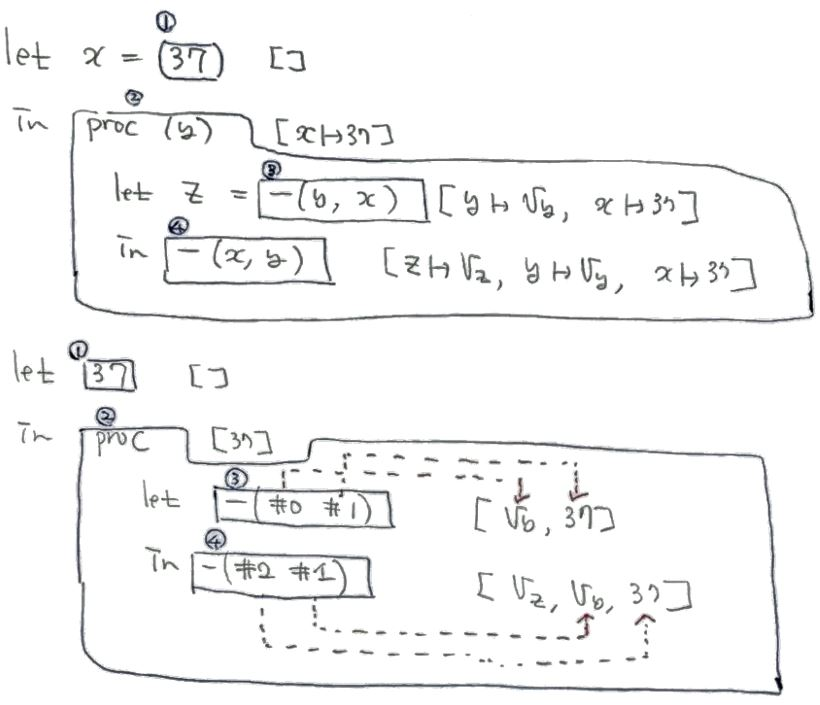
\includegraphics[width=0.75\linewidth]{fig_debruijn_indices}

%%%%%%%%%%%% Slide %%%%%%%%%%%%%%%%%%%%%%%%%%%%%%%%%%%%%%%%%%%%%%%%%%%
\heading{3.7 Implementing Lexical Addressing}

Implementation of the lexical address analysis: \al
let x = 37 \al
in proc (y) \al
\ \ \ let z = -(y,x) \ \ \ \ \ \ \ \ \ depth(y)=0, depth(x)=1 \al
\ \ \ in -(x,y) \ \ \ \ \ \ \ \ \ \ \ \ \ \ \ depth(x)=2, depth(y)=1 \al
\al
is translated into \al
\al
(a-program \al
\ \ \ (nameless-let-exp (const-exp 37) \al
\ \ \ (nameless-proc-exp \al
\ \ \ \ \ \ (nameless-let-exp \al
\ \ \ \ \ \ \ \ \ (diff-exp (nameless-var-exp 0) (nameless-var-exp 1)) \al
\ \ \ \ \ \ \ \ \ (diff-exp (nameless-var-exp 2) (nameless-var-exp 1)) \al

%%%%%%%%%%%% Slide %%%%%%%%%%%%%%%%%%%%%%%%%%%%%%%%%%%%%%%%%%%%%%%%%%%
\heading{3.7.1 The Translator}

A procedure translation-of-program that \al
- takes a program, \al
- removes all the variables from the declarations, and \al
- replaces every variable reference by its lexical depth.

cf. translation-of-program vs. value-of-program

Static environment: a list of variables, representing the scopes within
which the current expression lies. \al
- See Figure 3.15 \al
- cf. Senv vs. Env

Implementation: P.96 and Figure 3.16

%%%%%%%%%%%% Slide %%%%%%%%%%%%%%%%%%%%%%%%%%%%%%%%%%%%%%%%%%%%%%%%%%%
\heading{3.7.2 The Nameless Interpreter}

This interpreter takes advantage of the predictions of the lexical-address
analyzer to avoid explicitly searching for variables at runtime.

Nameless environment: a list of denoted values \al
- Figure 3.17 and the figure in P.98

Two modified procedures, value-of and value-of-program, 
with nameless environment \al
- Figure 3.18 and P.100

\end{huge}
\end{document}





